\documentclass[10pt]{ctexart}
\usepackage{listings}
\usepackage{amsmath} 
\usepackage{amssymb} 
\usepackage{xcolor}
\usepackage{xeCJK}
\usepackage{fontspec}
\usepackage{titlesec}
\usepackage{titletoc}
\usepackage{setspace}
\usepackage{graphicx}
\usepackage{geometry}
\usepackage[T1]{fontenc}  
\usepackage{textcomp}
\usepackage{lmodern}
%\usepackage{caption}
\usepackage[justification=centering]{subcaption}
\usepackage[justification=centering]{caption}
\usepackage{tikz}
\usetikzlibrary{graphs}
\usepackage{amsfonts}
\usepackage[colorlinks,
            linkcolor=black,
            anchorcolor=black,
            citecolor=black]{hyperref}
\geometry{a4paper,scale=0.8}
\renewcommand\contentsname{Contents}
%\setmonofont[Mapping={}]{Monaco}    %英文引号之类的正常显示,相当于设置英文字体
%\setsansfont{Consolas} %设置英文字体 Monaco, Consolas,  Fantasque Sans Mono
%\setmainfont{Monaco} %设置英文字体
\setmonofont{Consolas}
% 定义可能使用到的颜色
%\setmainfont[BoldFont=SimHei]{SimSun}
\definecolor{CPPLight}  {HTML} {686868}
\definecolor{CPPSteel}  {HTML} {888888}
\definecolor{CPPDark}   {HTML} {262626}
\definecolor{CPPBlue}   {HTML} {4172A3}
\definecolor{CPPGreen}  {HTML} {487818}
\definecolor{CPPBrown}  {HTML} {A07040}
\definecolor{CPPRed}    {HTML} {AD4D3A}
\definecolor{CPPViolet} {HTML} {7040A0}
\definecolor{CPPGray}  {HTML} {B8B8B8}
\lstset{
    columns=fixed,       
    % numbers=left,                                        % 在左侧显示行号
    frame=none,                                          % 不显示背景边框
    backgroundcolor=\color[RGB]{245,245,244},            % 设定背景颜色
    keywordstyle=\color[RGB]{40,40,255},                 % 设定关键字颜色
    numberstyle=\small\color{darkgray},                  % 设定行号格式
    commentstyle=\it\color[RGB]{0,96,96},                % 设置代码注释的格式
    stringstyle=\rmfamily\slshape\color[RGB]{128,0,0},   % 设置字符串格式
    showstringspaces=false,                              % 不显示字符串中的空格
    language=c++,                                        % 设置语言
    morekeywords={alignas,continute,friend,register,true,alignof,decltype,goto,
    reinterpret_cast,try,asm,defult,if,return,typedef,auto,delete,inline,short,
    typeid,bool,do,int,signed,typename,break,double,long,sizeof,union,case,
    dynamic_cast,mutable,static,unsigned,catch,else,namespace,static_assert,using,
    char,enum,new,static_cast,virtual,char16_t,char32_t,explict,noexcept,struct,
    void,export,nullptr,switch,volatile,class,extern,operator,template,wchar_t,
    const,false,private,this,while,constexpr,float,protected,thread_local,
    const_cast,for,public,throw,std},
    emph={map,set,multimap,multiset,unordered_map,unordered_set,
    unordered_multiset,unordered_multimap,vector,string,list,deque,
    array,stack,forwared_list,iostream,memory,shared_ptr,unique_ptr,
    random,bitset,ostream,istream,cout,cin,endl,move,default_random_engine,
    uniform_int_distribution,iterator,algorithm,functional,bing,numeric,},
    emphstyle=\color{CPPViolet},
    basicstyle=\linespread{1}\small\fontspec{Consolas}\ttfamily,
    breaklines=true,
    %xleftmargin=1em,xrightmargin=1em, aboveskip=1em,
    % in the listings package configuration, try:  
    literate={"}{\textquotedbl}1,  
    tabsize=4, keepspaces=true
}
\CTEXoptions[today=old]
\title{Exercises 7}
\author{软件工程一班 \ 张逸松 57号}
\date{\today}

\begin{document}
    \maketitle
    \subsection*{1.2}
    \begin{itemize}
        \item [\textbf{a)}] a;
        \item [\textbf{b)}] a, b, c, d, f, h, j, q, t;
        \item [\textbf{c)}] e, g, i, k, l, m, n, o, p, r, s, u;
        \item [\textbf{d)}] q, r;
        \item [\textbf{e)}] c;
        \item [\textbf{f)}] p;
        \item [\textbf{g)}] f, b, a;
        \item [\textbf{h)}] e, f, l, m, n;
    \end{itemize}
    \subsection*{1.10}
    2000 edges.
    \subsection*{1.14}
    A \textbf{complete $m$-ary tree} is a full $m$-ary tree in which every leaf is at the same level. \par
    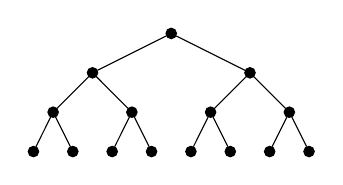
\begin{tikzpicture}
        \node (1) at (0, 0) [circle , draw, fill = black, scale = 0.4pt] {};
        \node (2) at (0.5, 0) [circle , draw, fill = black, scale = 0.4pt] {};
        \node (3) at (1, 0) [circle , draw, fill = black, scale = 0.4pt] {};
        \node (4) at (1.5, 0) [circle , draw, fill = black, scale = 0.4pt] {};
        \node (5) at (2, 0) [circle , draw, fill = black, scale = 0.4pt] {};
        \node (6) at (2.5, 0) [circle , draw, fill = black, scale = 0.4pt] {};
        \node (7) at (3, 0) [circle , draw, fill = black, scale = 0.4pt] {};
        \node (8) at (3.5, 0) [circle , draw, fill = black, scale = 0.4pt] {};
        \node (9) at (0.25, 0.5) [circle , draw, fill = black, scale = 0.4pt] {};
        \node (10) at (1.25, 0.5) [circle , draw, fill = black, scale = 0.4pt] {};
        \node (11) at (2.25, 0.5) [circle , draw, fill = black, scale = 0.4pt] {};
        \node (12) at (3.25, 0.5) [circle , draw, fill = black, scale = 0.4pt] {};
        \node (13) at (0.75, 1) [circle , draw, fill = black, scale = 0.4pt] {};
        \node (14) at (2.75, 1) [circle , draw, fill = black, scale = 0.4pt] {};
        \node (15) at (1.75, 1.5) [circle , draw, fill = black, scale = 0.4pt] {};
        \draw [] (15) edge (14);
        \draw [] (15) edge (13);
        \draw [] (14) edge (12);
        \draw [] (14) edge (11);
        \draw [] (13) edge (10);
        \draw [] (13) edge (9);
        \draw [] (12) edge (8);
        \draw [] (12) edge (7);
        \draw [] (11) edge (6);
        \draw [] (11) edge (5);
        \draw [] (10) edge (4);
        \draw [] (10) edge (3);
        \draw [] (9) edge (2);
        \draw [] (9) edge (1);
    \end{tikzpicture}
    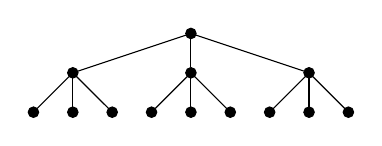
\begin{tikzpicture}
        \node (1) at (0, 0) [circle , draw, fill = black, scale = 0.4pt] {};
        \node (2) at (0.5, 0) [circle , draw, fill = black, scale = 0.4pt] {};
        \node (3) at (1, 0) [circle , draw, fill = black, scale = 0.4pt] {};
        \node (4) at (1.5, 0) [circle , draw, fill = black, scale = 0.4pt] {};
        \node (5) at (2, 0) [circle , draw, fill = black, scale = 0.4pt] {};
        \node (6) at (2.5, 0) [circle , draw, fill = black, scale = 0.4pt] {};
        \node (7) at (3, 0) [circle , draw, fill = black, scale = 0.4pt] {};
        \node (8) at (3.5, 0) [circle , draw, fill = black, scale = 0.4pt] {};
        \node (9) at (4, 0) [circle , draw, fill = black, scale = 0.4pt] {};
        \node (10) at (0.5, 0.5) [circle , draw, fill = black, scale = 0.4pt] {};
        \node (11) at (2, 0.5) [circle , draw, fill = black, scale = 0.4pt] {};
        \node (12) at (3.5, 0.5) [circle , draw, fill = black, scale = 0.4pt] {};
        \node (13) at (2, 1) [circle , draw, fill = black, scale = 0.4pt] {};
        \draw [] (1) edge (10);
        \draw [] (2) edge (10);
        \draw [] (3) edge (10);
        \draw [] (4) edge (11);
        \draw [] (5) edge (11);
        \draw [] (6) edge (11);
        \draw [] (7) edge (12);
        \draw [] (8) edge (12);
        \draw [] (9) edge (12);
        \draw [] (10) edge (13);
        \draw [] (11) edge (13);
        \draw [] (12) edge (13);
    \end{tikzpicture}
    \subsection*{2.1}
    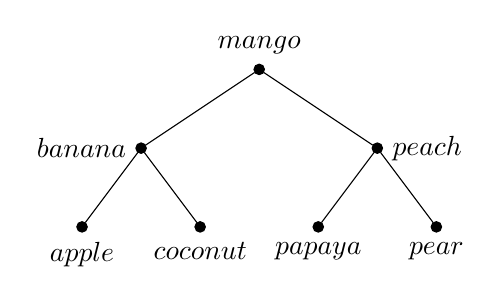
\begin{tikzpicture}
        \node (1) at (0, 0) [circle , draw, fill = black, label=below:$apple$, scale = 0.4pt] {};
        \node (2) at (0.75, 1) [circle , draw, fill = black,label=left:$banana$,  scale = 0.4pt] {};
        \node (3) at (1.5, 0) [circle , draw, fill = black,label=below:$coconut$,  scale = 0.4pt] {};
        \node (4) at (2.25, 2) [circle , draw, fill = black,label=above:$mango$,  scale = 0.4pt] {};
        \node (5) at (3, 0) [circle , draw, fill = black,label=below:$papaya$,  scale = 0.4pt] {};
        \node (6) at (3.75, 1) [circle , draw, fill = black,label=right:$peach$,  scale = 0.4pt] {};
        \node (7) at (4.5, 0) [circle , draw, fill = black,label=below:$pear$,  scale = 0.4pt] {};
        \draw [] (1) edge (2);
        \draw [] (2) edge (4);
        \draw [] (3) edge (2);
        \draw [] (5) edge (6);
        \draw [] (6) edge (4);
        \draw [] (7) edge (6);
    \end{tikzpicture}
    \subsection*{2.4}
    We need to weigh twice. \par
    First, choose any two coin, weigh them. \par
    Second, if two coin are as heavy, that means the fake coin is among the two remaining coins, weigh again. If two coin are not the same weight, choose any one of them and any one of remaining, weigh. If they are the same, the remaining of first step are fake. Otherwise, that this time is fake.
\end{document}